\chapter{Sistema Embebido}
\cleanchapterquote{No me dan miedo los ordenadores. Temo la falta de ellos}{Isaac Asimov}{(Escritor americano)}

En este capitulo se abordan los procedimientos de diseño del sistema embebido desde la parte mecánica hasta la
obtención del controlador.

\section{Arquitectura}
La arquitectura general del sistema embebido está dividido en 3 diferentes sub-áreas que en su conjunto ayudan al
seguimiento de un objetivo mediante visión artificial.
\begin{center}
	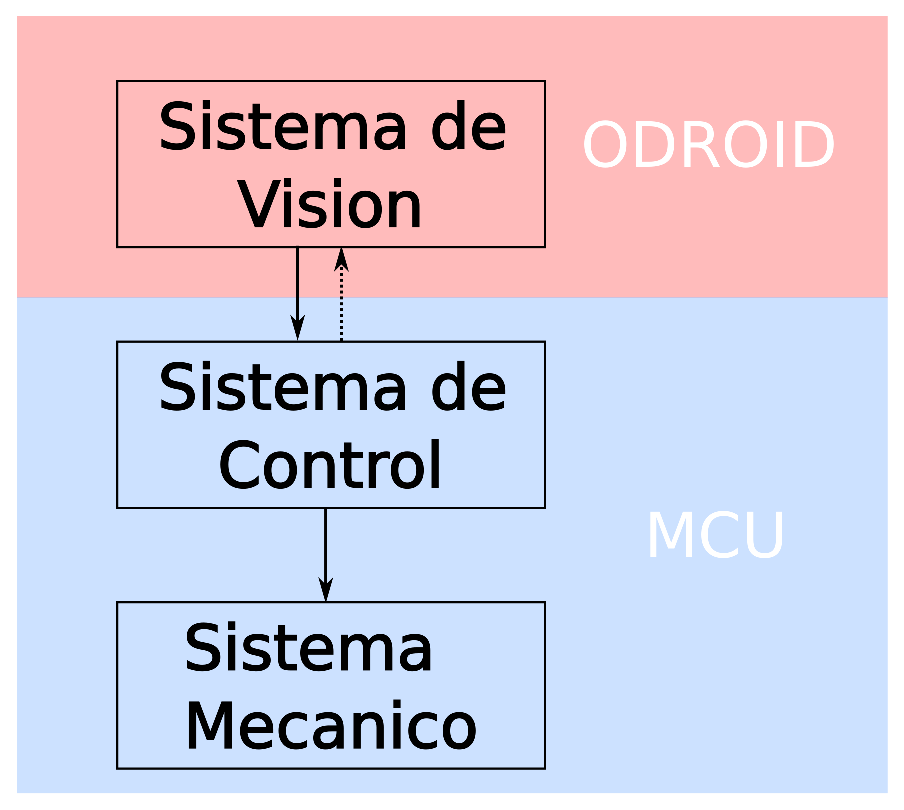
\includegraphics[width=0.45\textwidth]{Contenido/Cuerpo/Capitulo5/Fig12.eps}
	\captionof{figure}{Modulos del sistema}\label{Fig1}
\end{center}
Tal y como se ilustra en la figura 5.1, dichas áreas se relacionan entre si, compartiendo datos para tener un
sistema integrado y robusto.
\begin{itemize}
	\item Visión: Identifica el centroide del objetivo, el desarrollo del algoritmo se abordó en el capítulo 4. Interacciona con el sistema de control enviando la retroalimentación
	      y recibe de este ultimo datos del error.
	\item Control: Un micro-controlador es el encargado de interactuar con los datos de la cámara y retroalimentarlos con la
	      salida deseada, para después controlar con un PI.
	\item Mecánico: Son los actuadores del sistema que hacen que la cámara tenga dos grados de libertad de movimiento, que
	      son las rotaciones en Pitch y Yaw, el modelo se abordó en el Capitulo 3.
\end{itemize}
La comunicación de datos se da por varios buses de datos, entre todos los componentes del sistema, la figura 5.2 ilustra
la interacción entre ellos y se presenta la arquitectura propuesta
\begin{center}
	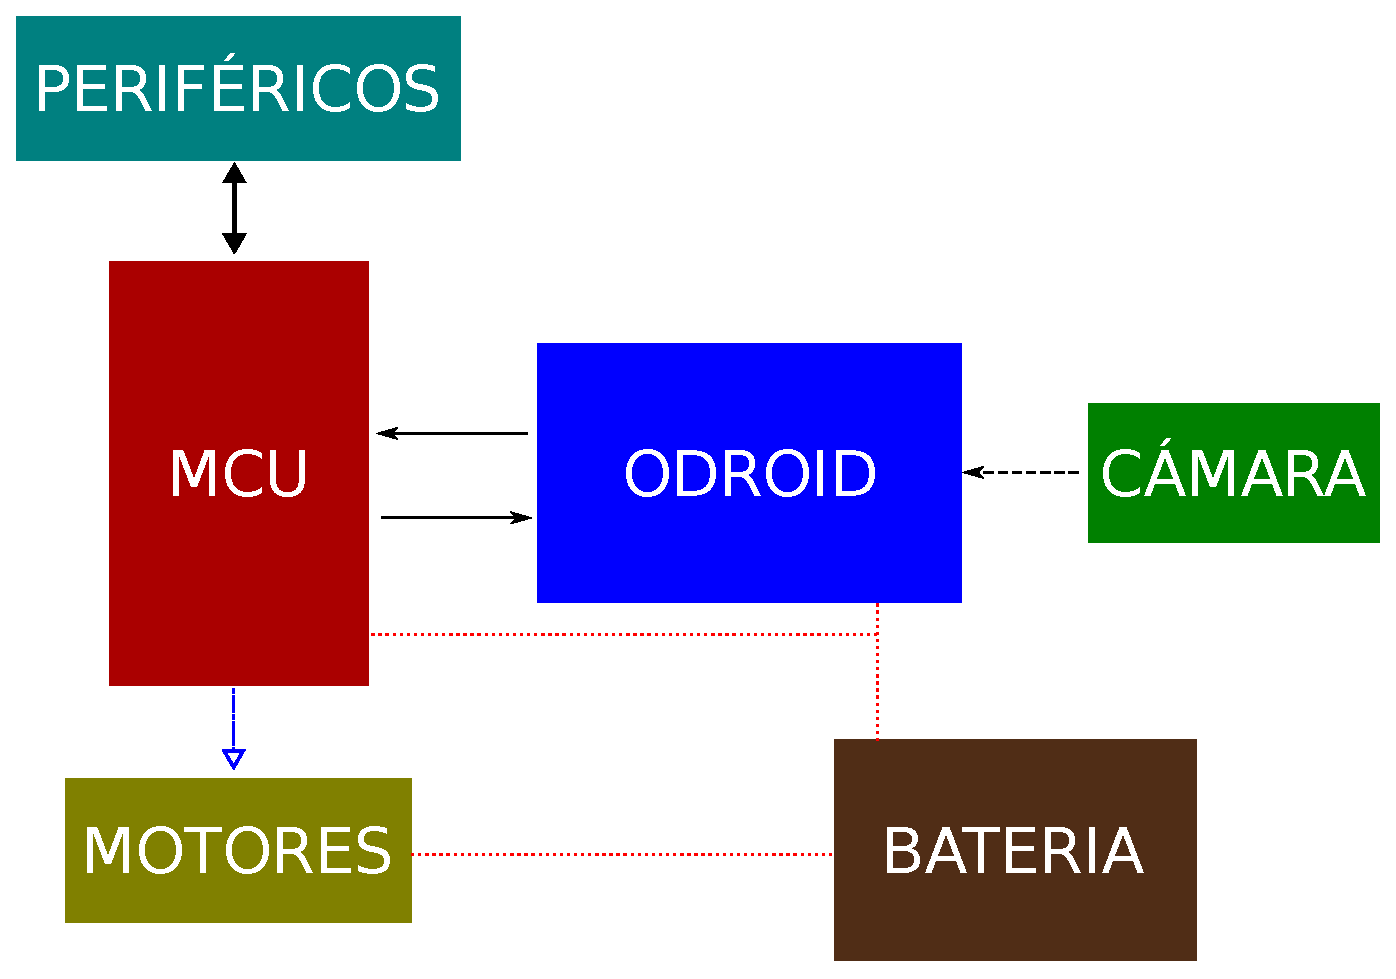
\includegraphics[width=0.5\textwidth]{Contenido/Cuerpo/Capitulo5/Fig13.eps}
	\captionof{figure}{Arquitectura del sistema}\label{Fig1}
\end{center}
El microcontrolador es de 32 bits arquitectura RISC, las especificaciones detalladas de los motores y de la tarjeta de desarrollo
ODROID puede ser consultada en el Apéndice B.\\
El Bus señalado con líneas punteadas en rojo representan la conexión de voltaje con los demás componentes, mientras que la línea punteada en negro entre la cámara y la odroid
simboliza la conexión USB para la transferencia de datos, la comunicación entre ODROID y el MCU se da mediante el módulo RS-323 integrado en el microcontrolador que a su vez
se comunica con los periféricos deseados utilizando sus salidas digitales.\\
Este tipo de Arquitectura permite que la ODROID pueda comunicarse paralelamente con el MCU por medio del protocolo serial, que va
a 57000 baudios, además de que permite que el microcontrolador tenga la posibilidad de publicar en ROS.

% ---------------------------------------------------------------------------------------------------------
% *********************************************************************************************************
% *********************************************************************************************************
% ---------------------------------------------------------------------------------------------------------


\section{Mecanismo móvil}
El diseño del sistema fue hecho mediante el uso de software libre llamado OpenSCAD, en el cual se trazó el prototipo del
sistema utilizando dos motores tipo servo, es decir, que tienen su propio controlador de velocidad integrado vía PWM.
\begin{center}
	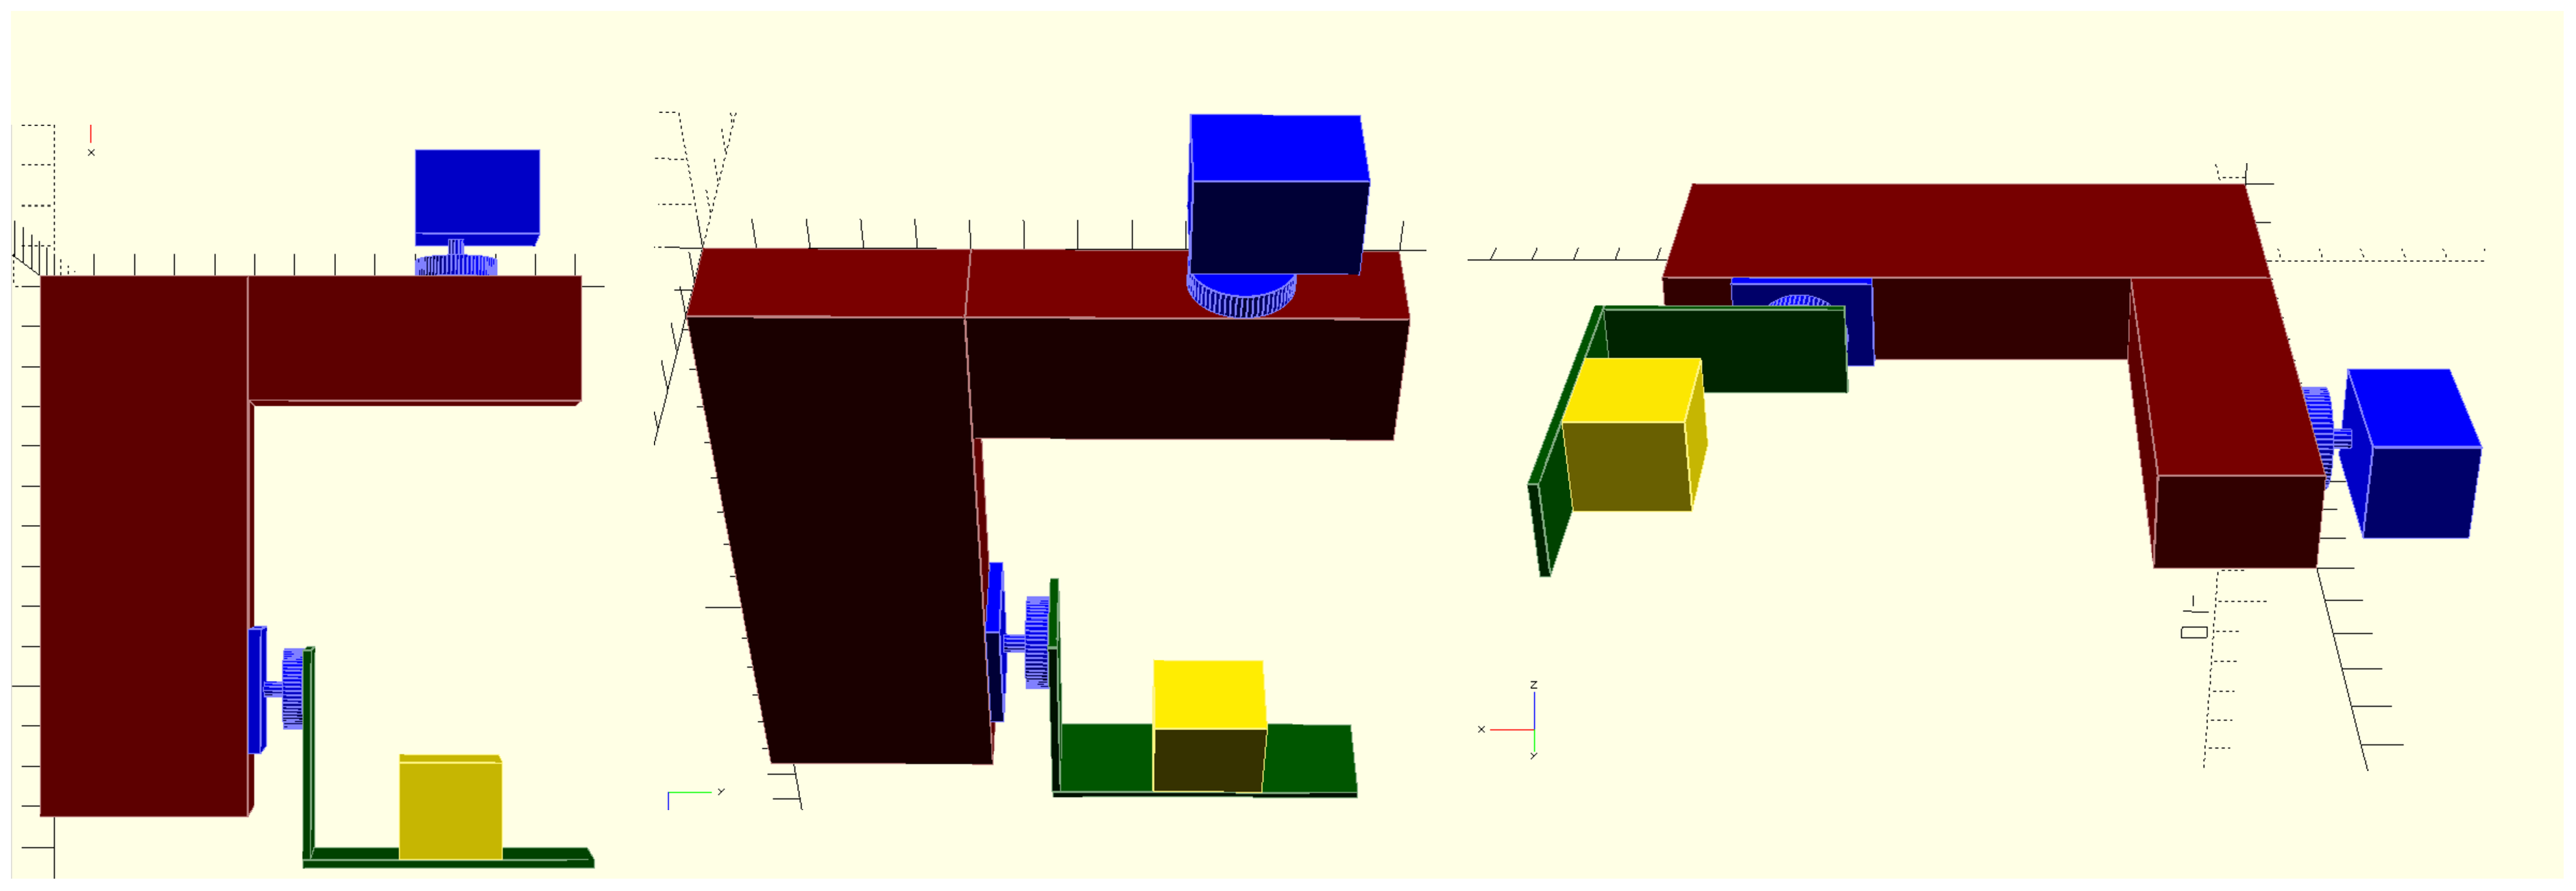
\includegraphics[width=1.0\textwidth]{Contenido/Cuerpo/Capitulo5/Fig14.eps}
	\captionof{figure}{Diseño CAD del prototipo}\label{Fig1}
\end{center}
En la figura 5.3 los motores están representados en color azul, mientras que la cámara esta de amarillo, como se puede apreciar
la cámara recae sobre un soporte de color verde, dicha cámara está sujeta por un par de ligas que ayudan a que esta no se
caiga cuando hay rotación en pitch\\
A continuación en la figura 5.4 se presentan algunas medidas del diseño, las unidades están en mm.
\begin{center}
	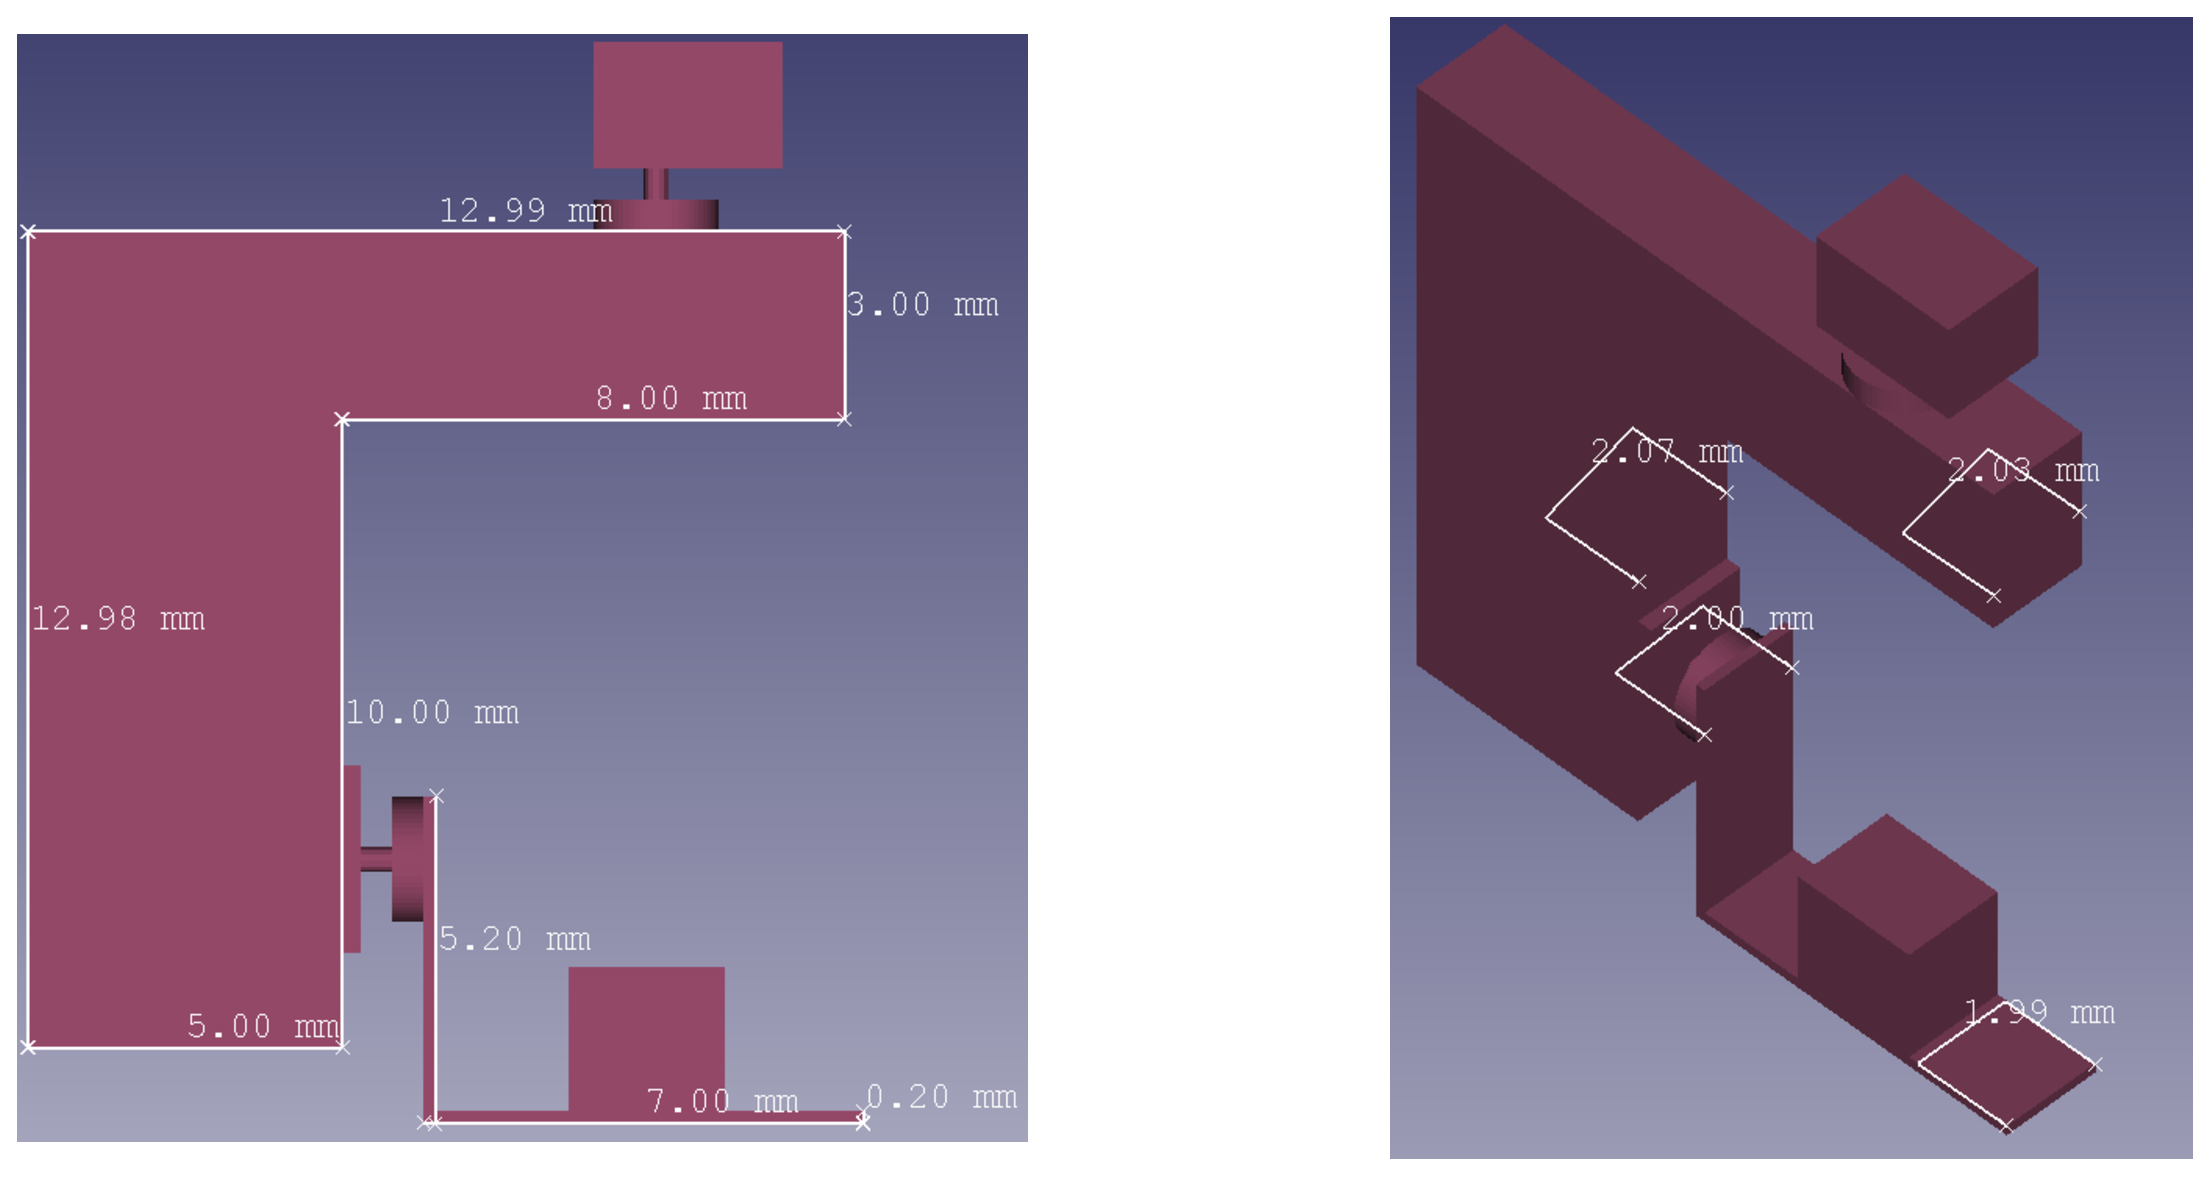
\includegraphics[width=0.8\textwidth]{Contenido/Cuerpo/Capitulo5/Fig16.eps}
	\captionof{figure}{Dimensiones del CAD}\label{Fig1}
\end{center}
Como se vio previamente en los capítulos 2 y 3 este sistema tendrá dos ejes de libertad, que en términos técnicos, a estos
movimientos también se les conoce como "\ Till \" y "\ Pan \" que es no es mas que otra manera de decirle a la rotación
sobre el eje Y y Z.\\
Es entonces que esos movimientos pueden ser visualizados como se presenta en la figura 5.5.
\begin{center}
	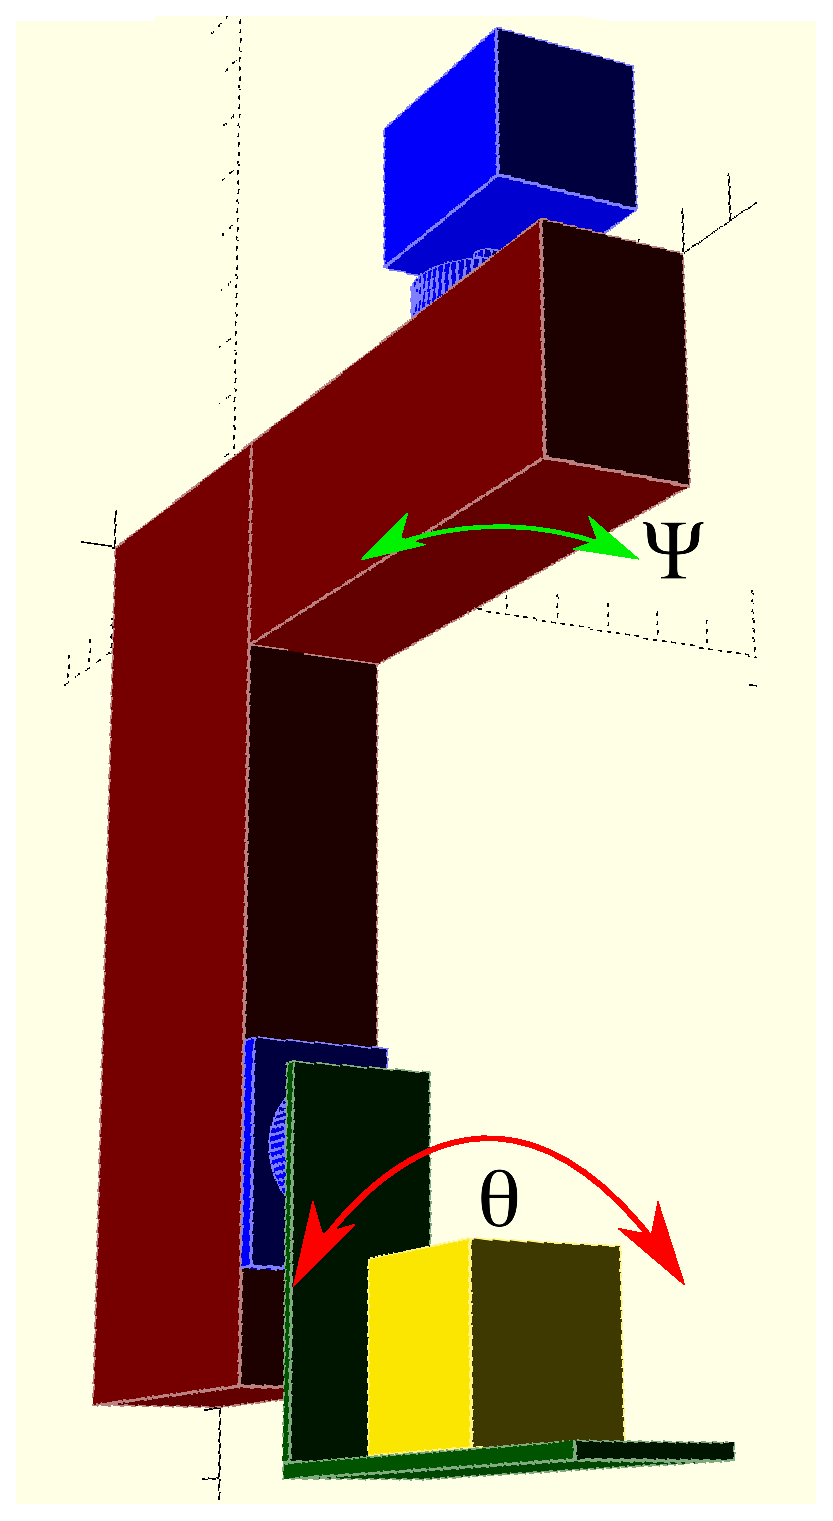
\includegraphics[width=0.35\textwidth]{Contenido/Cuerpo/Capitulo5/Fig15.eps}
	\captionof{figure}{Grados de libertad del sistema}\label{Fig1}
\end{center}
Donde
\begin{itemize}
	\item $\theta$ representa el movimiento de "\ Till "
	\item $\psi$ representa el movimiento de "\ Pan  "
\end{itemize}

% ---------------------------------------------------------------------------------------------------------
% *********************************************************************************************************
% *********************************************************************************************************
% ---------------------------------------------------------------------------------------------------------
\section{Prototipo físico}
Para la realización del prototipo se utilizó un material ligero para que no agregue mucho peso adicional al sistema.
\begin{center}
	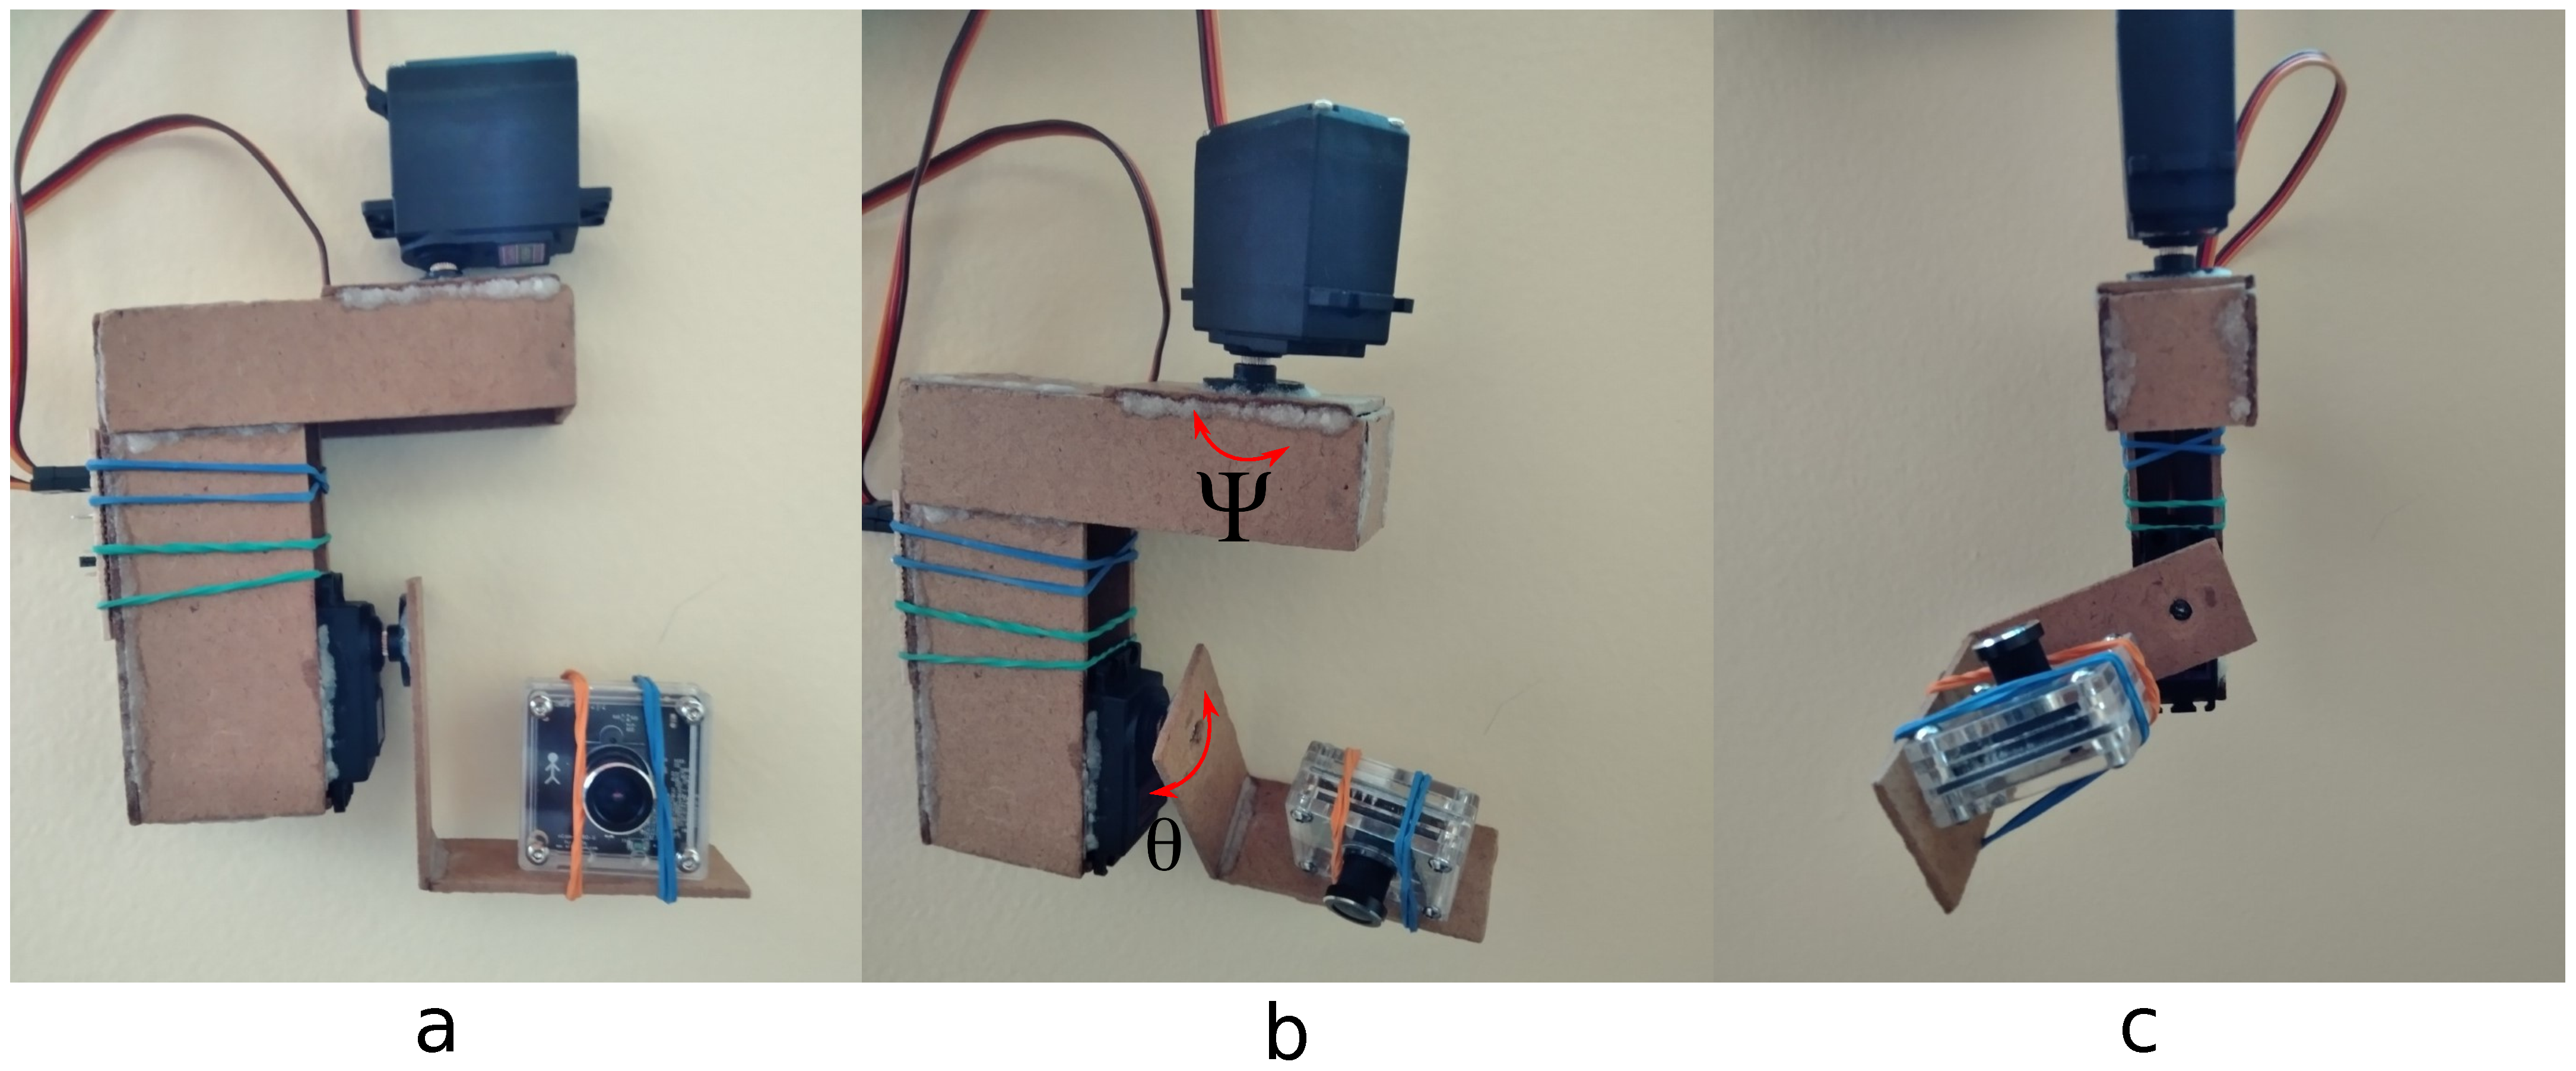
\includegraphics[width=0.8\textwidth]{Contenido/Cuerpo/Capitulo5/Fig17.eps}
	\captionof{figure}{Prototipo del sistema hecho con madera}\label{Fig1}
\end{center}
Como se puede observar en la figura 5.6 la cámara esta sujeta a la base por medio de ligas que le dan mejor soporte y ayudan a que
esta no se caiga al momento de seguir a los objetivos.
\begin{itemize}
	\item Peso del sistema sin motores ni cámara : 70 g
	\item Peso con motores y cámara : 215 g
\end{itemize}
En b) y c) de la figura 5.6 se ilustra el movimiento que puede realizar el sistema, y que será controlado
por la cámara y actuado por los motores.\\
Adicionalmente se diseñó un pequeño circuito que sirve como terminal para las conexiones de alimentación y señales,
dicho circuito se encuentra en la parte lateral del sistema sujetado por ligas y pegamento.\\
La conexiones eléctricas se ilustra en la figura 5.7. Es una esquemático que muestra la conexión entre los componentes principales: la cámara(OCAM), monoprocesador(ODROID),
el microcontrolador (ATMEGA) y los motores (Servomotores)
\begin{center}
	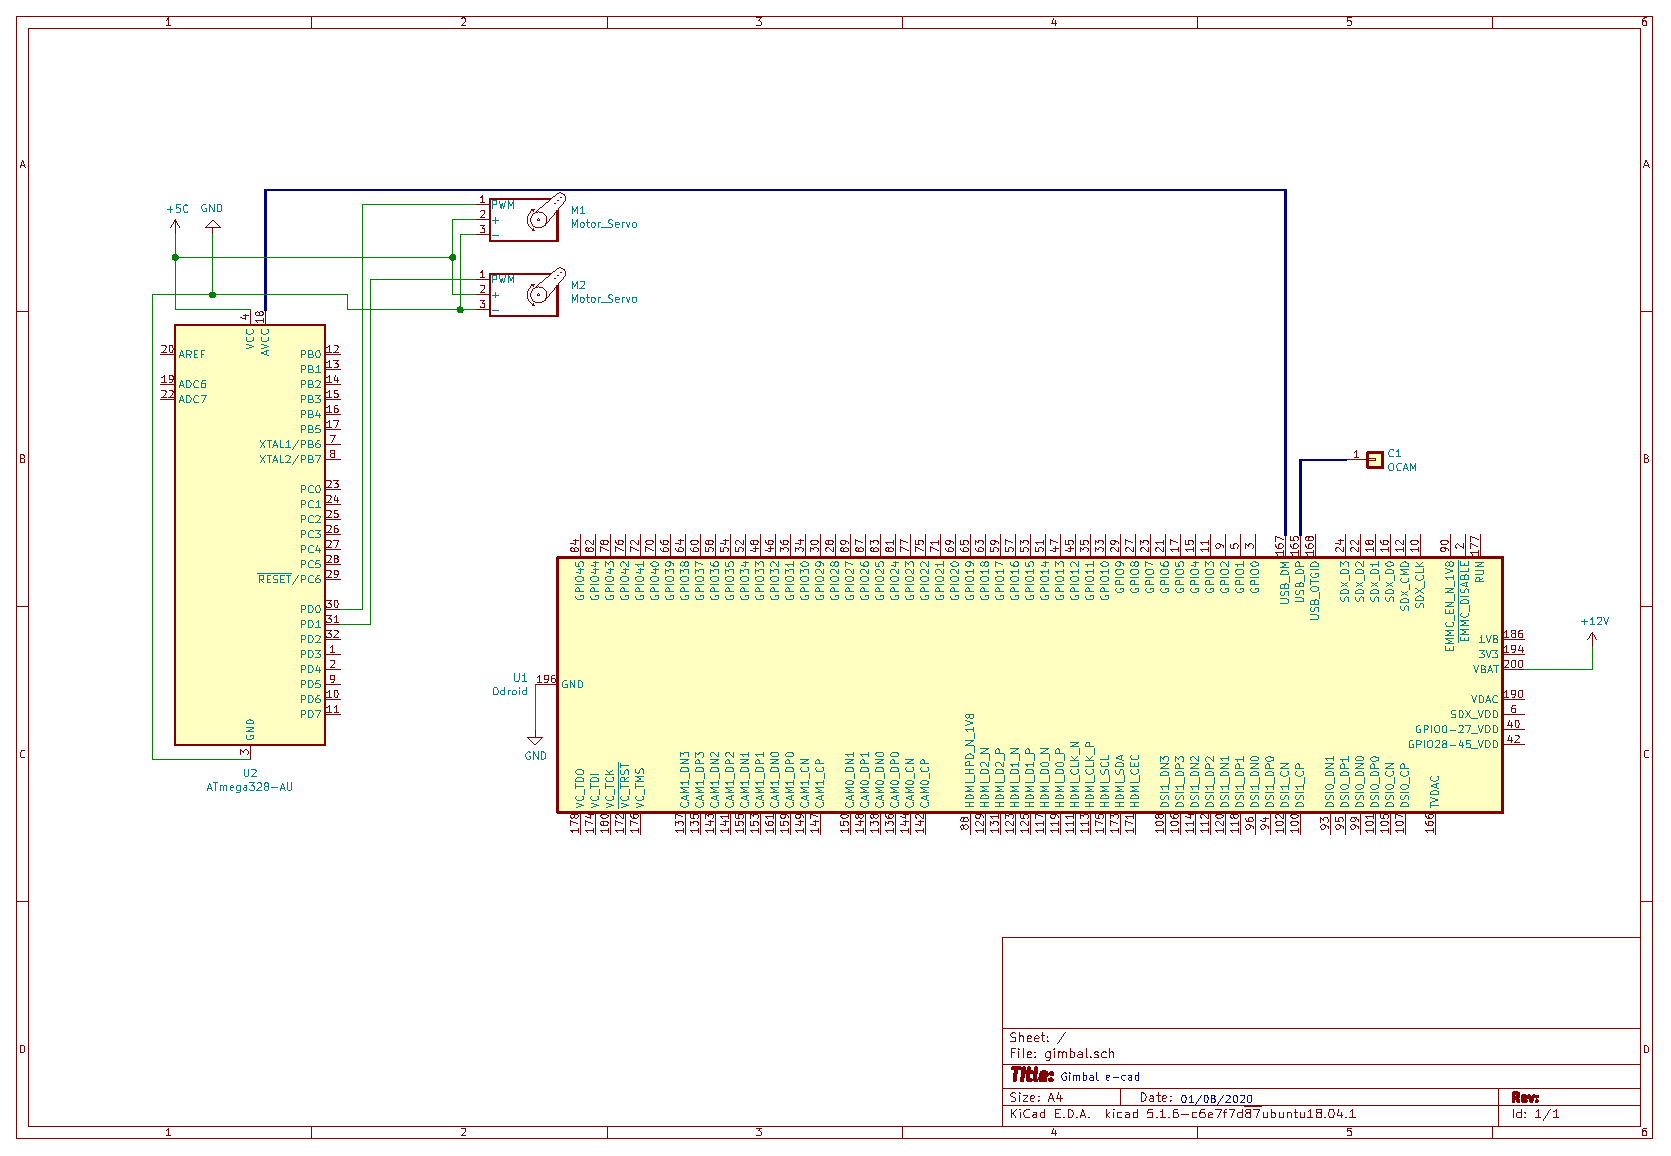
\includegraphics[width=1.0\textwidth]{Contenido/Cuerpo/Capitulo5/Fig21.eps}
	\captionof{figure}{Circuito eléctrico}\label{Fig1}
\end{center}


% ---------------------------------------------------------------------------------------------------------
% *********************************************************************************************************
% *********************************************************************************************************
% ---------------------------------------------------------------------------------------------------------


\section{ROS-Microcontrolador}
La parte mecánica encargada de hacer mover la cámara alrededor de dos ejes son los motores de corriente directa, que están conectados
a un microcontrolador que es el encargado de ejecutar el controlador.\\
El control tiene como entrada las coordenadas obtenidas por el algoritmo descrito en el capitulo 4. Y con base en ese pixel, podemos
calcular el error teniendo en cuenta que la referencia es el centro de la cámara.\\
Una vez dicho lo anterior queda una pregunta clara, ¿Como comunicar el microcontrolador encargado de los motores, con la cámara que
esta siendo ejecutada en ROS?
\begin{center}
	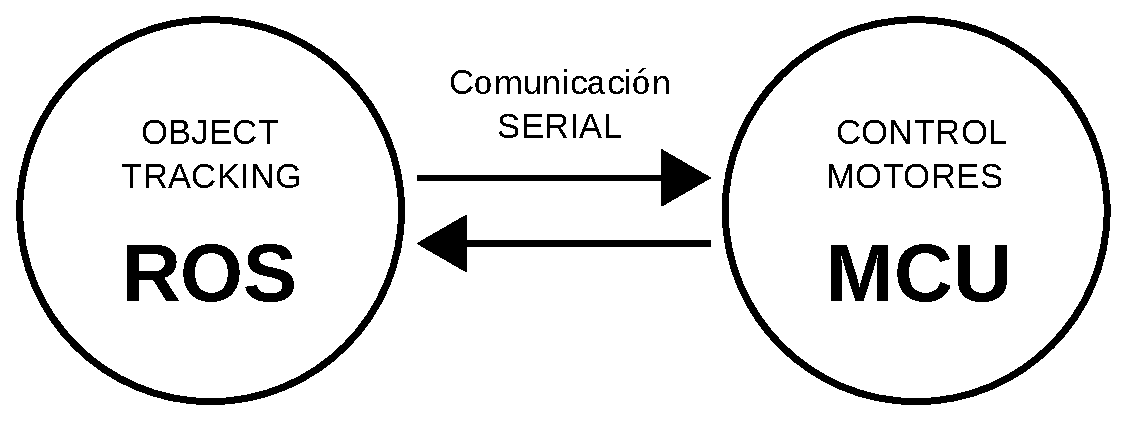
\includegraphics[width=0.45\textwidth]{Contenido/Cuerpo/Capitulo5/Fig1.eps}
	\captionof{figure}{Protocolo de comunicación}\label{Fig2}
\end{center}
Como se ilustra en la imagen anterior el protocolo de comunicación que se utilizó es el serial, debido a su practicad y que ya
cuenta con librerías de ROS para el microcontrolador, que para la primera etapa de esta investigación se utiliza el Atmega328p.\\
La comunicación esta basado en ser asíncrona, y se detalla mejor en el siguiente diagrama:
\begin{center}
	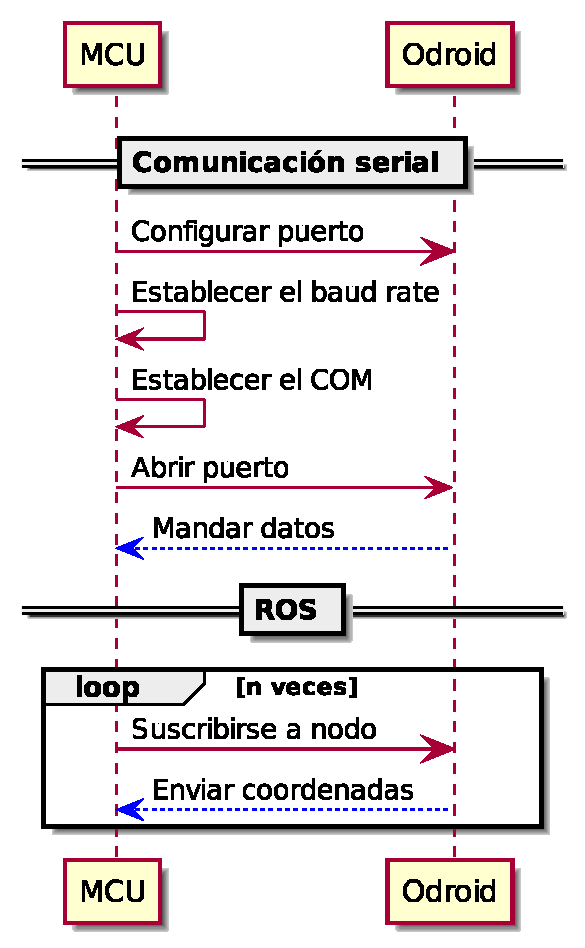
\includegraphics[width=0.35\textwidth]{Contenido/Cuerpo/Capitulo5/Fig2.eps}
	\captionof{figure}{Diagrama de secuencia}\label{Fig3}
\end{center}
La velocidad de la comunicación es de 570000 baudios y se conecta a través de un cable usb. El microcontrolador tiene además
la función de publicar el error con la finalidad de graficar dicho error y obtener conclusiones. Que visto desde el plano
de ROS tenemos los siguientes Topics y Nodes:
\begin{center}
	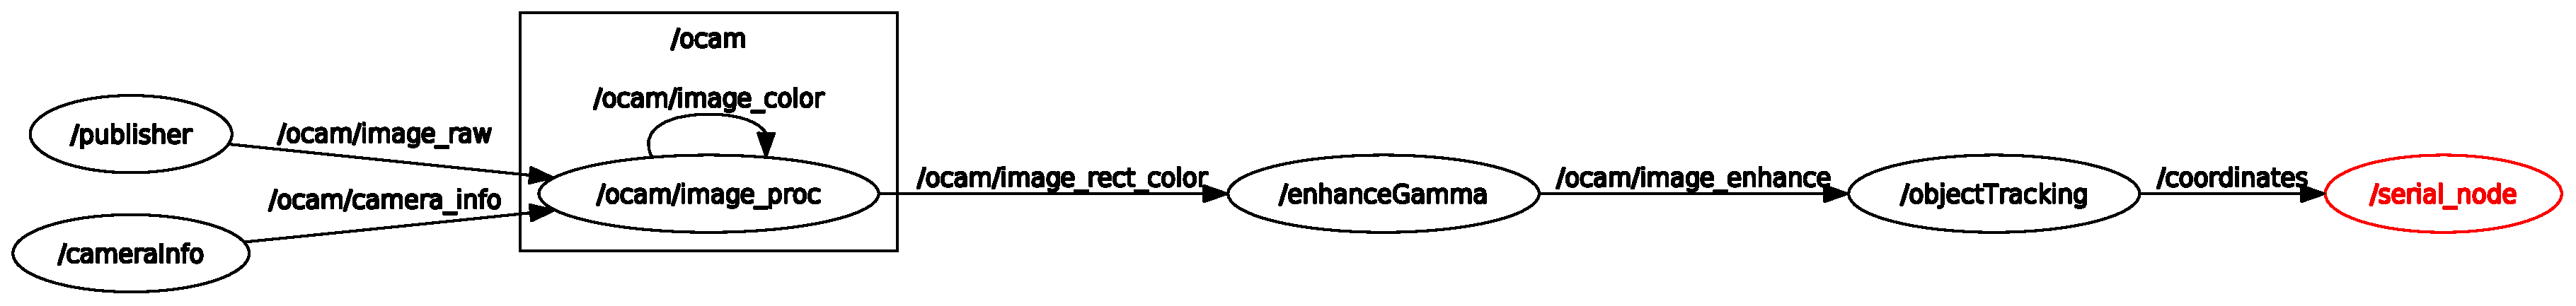
\includegraphics[width=0.9\textwidth]{Contenido/Cuerpo/Capitulo5/Fig3.eps}
	\captionof{figure}{Nodos y Topicos activos}\label{Fig4}
\end{center}


% ---------------------------------------------------------------------------------------------------------
% *********************************************************************************************************
% *********************************************************************************************************
% ---------------------------------------------------------------------------------------------------------


\section{Control}
La idea principal del sistema de control es la de encontrar una función de entrada $u(t)$ tal que la función de salida $x(t)$ siga a la
salida deseada $x^{des}(t)$. Para lograr esto vamos a utilizar la siguiente aproximación
\begin{equation}
	e(t) = x^{des}(t) - x(t)
\end{equation}
Donde $e(t)$ representa el error. Por lo que la estrategia es encontrar un $u(t)$ tal que
\begin{equation}
	\ddot{e} + k_v\dot{e} + k_pe = 0
\end{equation}
Donde $k_v$ y $k_p$ $> 0$\\
Y tal y como se abordo en el capitulo 2 esto nos lleva al control Proporcional-Derivativo
\begin{equation}
	u(t) = \ddot{x}^{des}(t) + k_v\dot{e}(t) + k_pe(t)
\end{equation}

La siguiente imagen ilustra el diagrama de bloques correspondiente al control del sistema para la coordenada X
\begin{center}
	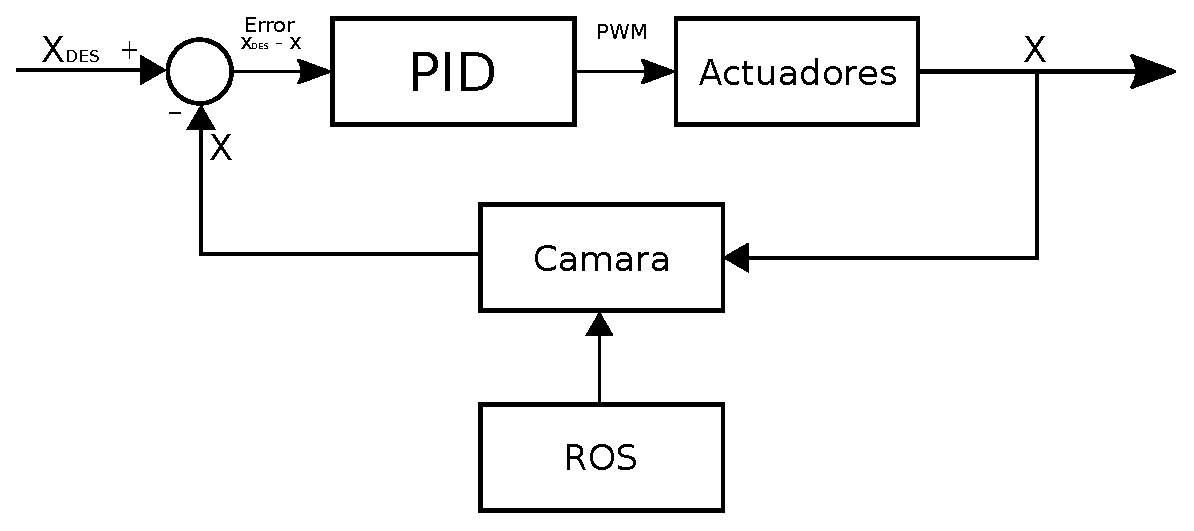
\includegraphics[width=0.6\textwidth]{Contenido/Cuerpo/Capitulo5/Fig6.eps}
	\captionof{figure}{Lazo de control}\label{Fig4}
\end{center}
Es un sistema de segundo orden retroalimentado por la camara y procesado en ROS. El lazo de control es aplicable también para la coordenada Y, como
fue abordado en la sección 5.4 la comunicación se da mediante
el protocolo serial, y debido a que la tarea que se encarga de realizar el algoritmo de control se debe suscribir al nodo de
coordenadas, este se ve limitado, a un tiempo de muestreo de 60fps, o dicho de otro modo a 16.66 ms.

\subsection{Función de tranferencia}
Como vimos en el capítulo 3, la función de transferencia de un motor de corriente continua es de segundo orden, e involucra algunas constantes que dependen del toque máximo y
de la velocidad sin carga.
\begin{equation}
	\frac{\theta_m (s)}{E_a(s)} = \frac{K_t / (R_aJ_m)}{s \left[ s + \frac{1}{J_m} \left( D_m + \frac{K_tK_b}{R_a} \right) \right]}
\end{equation}
El motor que se utilizó para hacer el mecanismo móvil es el MG996R, es un motor de tipo servo 360 grados, esto quiere decir que da todo el giro, a diferencia de los servomotores
convencionales. Las especificaciones técnicas son las siguientes:
\begin{itemize}
	\item Peso = 55g
	\item Torque stall = 11kg/cm a 6v
	\item Velocidad sin carga = 0.14s/ 60° a 6v
	\item Voltaje de operación = 4.8v a 7.2v
	\item Temperatura de operación = 0°C - 55°C
	\item PWM = 20ms (50Hz) de operación
\end{itemize}
La siguiente gráfica muestra la relación que hay entre el torque y la velocidad, que como se puede observar es lineal. Esta grafica se obtuvo con los datos sugeridos del
provedor.
\begin{center}
	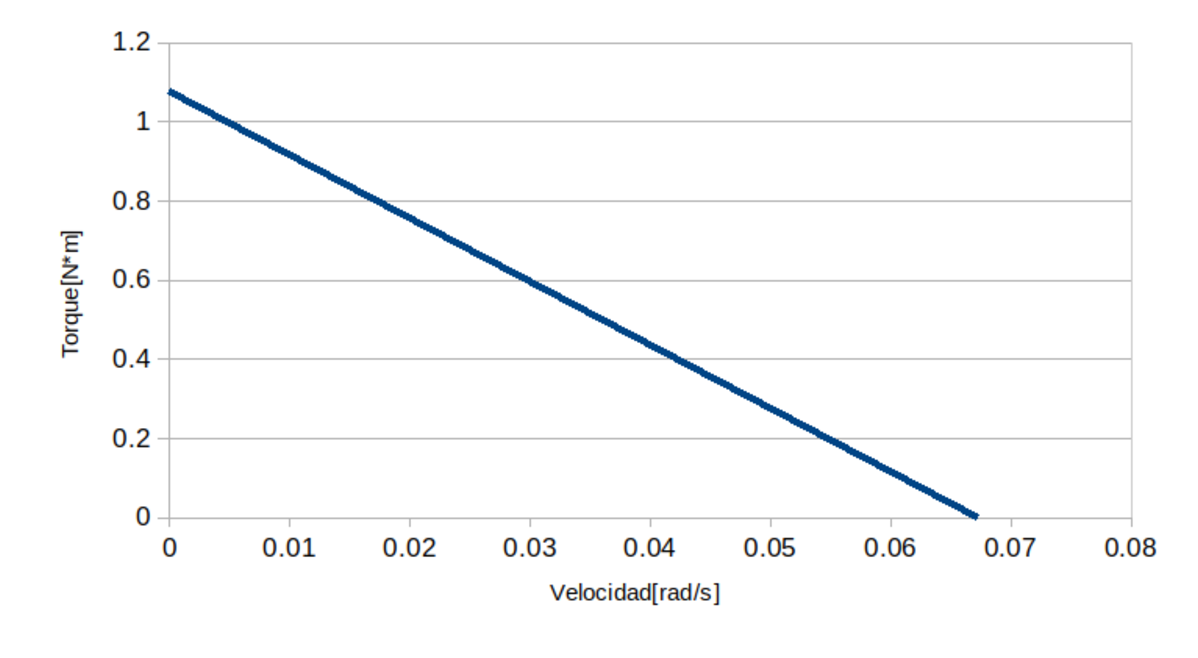
\includegraphics[width=0.8\textwidth]{Contenido/Cuerpo/Capitulo5/Fig19.eps}
	\captionof{figure}{Gráfica torque-velocidad}\label{Fig4}
\end{center}
Ahora encontraremos las constantes eléctricas, $K_t / R_a$ y $K_b$. De la curva de par-velocidad de la figura anterior
\begin{itemize}
	\item $T_{stall}$ = 1.078
	\item $\omega_{sincarga}$ = 0.0673
	\item $e_a$ = 6v
\end{itemize}
Las constantes electricas son
\begin{equation}
	\frac{K_t}{R_a} = \frac{T_{stall}}{e_a} = \frac{1.078}{6} = 0.17966
\end{equation}
y
\begin{equation}
	K_b = \frac{e_a}{\omega_{sin carga}} = \frac{6}{0.0673} = 89
\end{equation}
La carga en cada motor es diferente, vamos a calcularla con al siguiente ecuacion del momento de inercia
\begin{equation}
	I = mr^2
\end{equation}
\begin{center}
	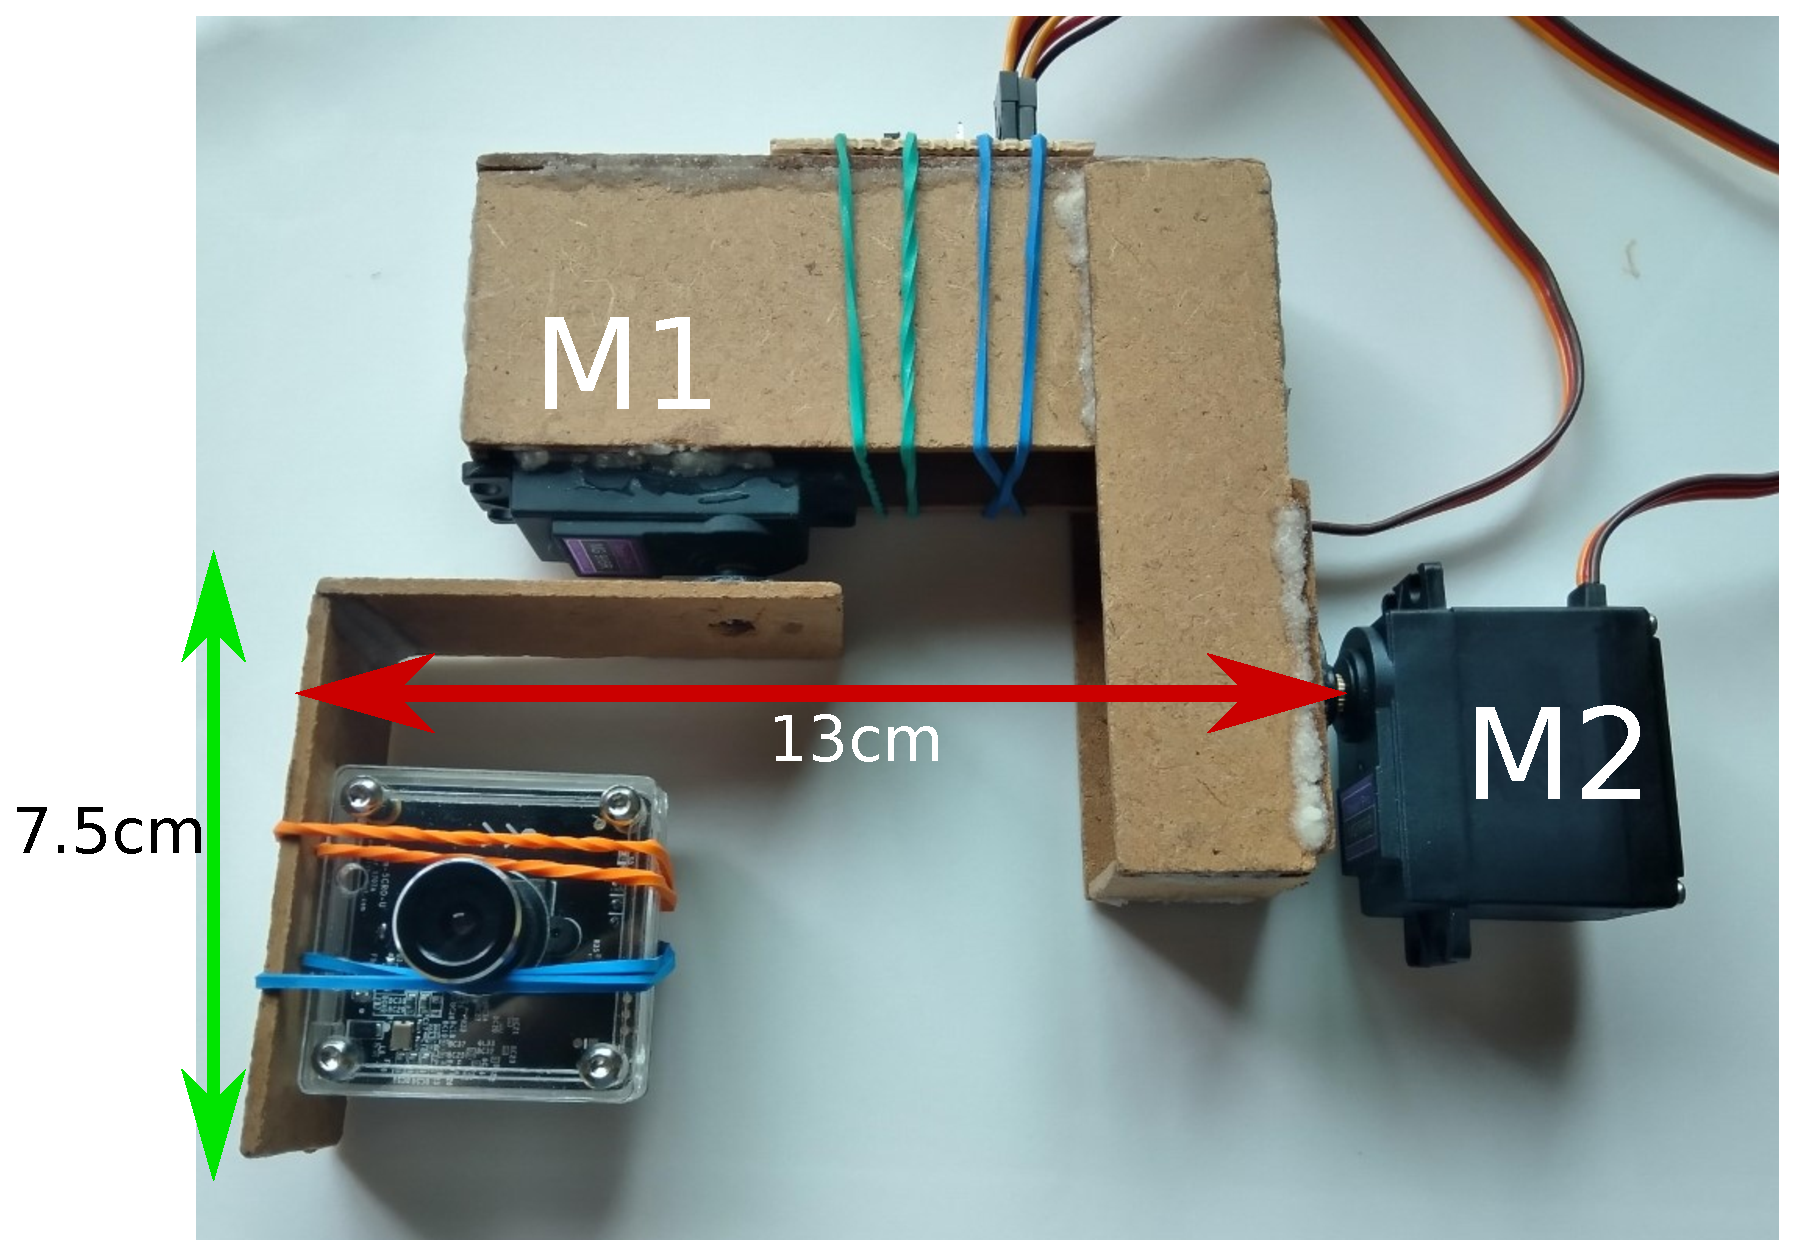
\includegraphics[width=0.6\textwidth]{Contenido/Cuerpo/Capitulo5/Fig20.eps}
	\captionof{figure}{Calculando momentos de inercia}\label{Fig4}
\end{center}
Para el motor 1 que en la imagen se identifica como M1 la distancia de actuación es de 7.5cm y lleva la carga de 35g de la cámara más 5g de la base. Por lo que aplicando
la ecuación anterior tenemos que
\begin{equation}
	I_1 = (40g)(3.75cm)^2 = 562.5g-cm^2 = 0.00005625 Kg-m^2
\end{equation}
Y para el motor 2 la masa es la acumulada de la masa1 + motor1 + estructura, dando como resultado 160 gramos
\begin{equation}
	I_2 = (160g)(6.5cm)^2 = 6760 g-cm^2 = 0.000676 kg-m^2
\end{equation}
De los valores para $J_m$ de motores de correinte continua comerciales tenemos un rango de 0.0000014 - 0.00005 $kg-m^2$

Debido a lo pequeño de estos valores, podemos hacer 0 a la variable $J_m$, por lo que la función de transferencia queda
\begin{equation}
	\frac{\theta_m (s)}{E_a(s)} = \frac{K_t / R_a}{s \left[ s +  \left( \frac{K_tK_b}{R_a} \right) \right]} = \frac{0.17966}{s(s+16)}
\end{equation}

\subsection{Algortimo de control}
El algoritmo general del control esta descrito en los siguientes diagramas, basado en programación orientado a objetos
donde hay dos puntos claves, la obtención de datos y la publicación de los errores para después ser graficados.
\begin{center}
	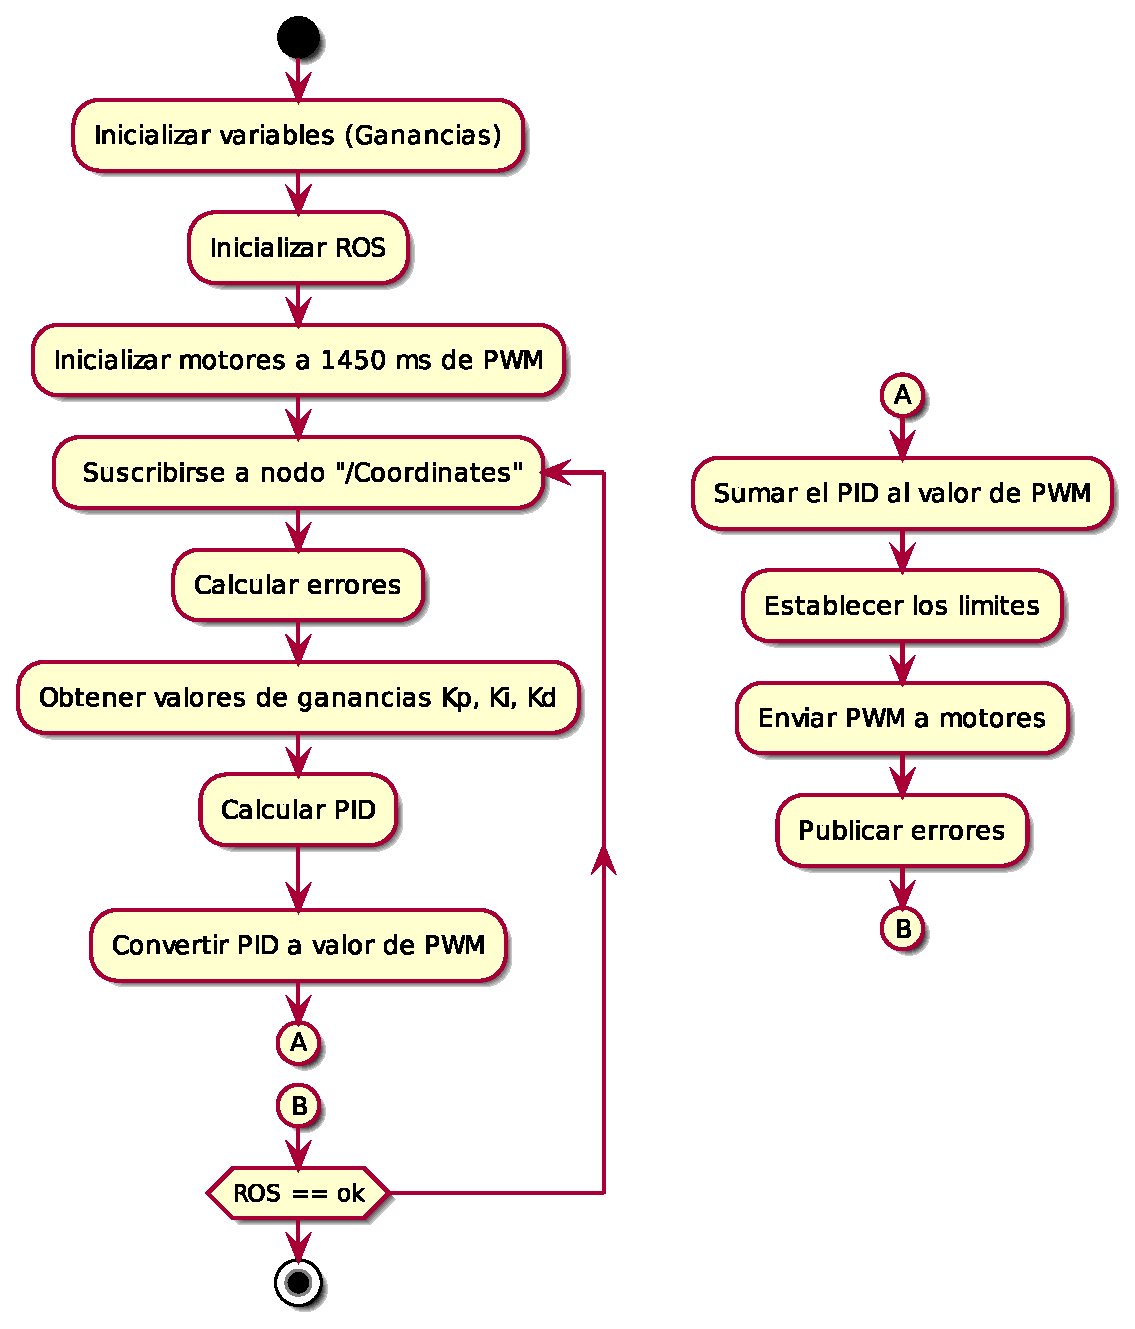
\includegraphics[width=0.6\textwidth]{Contenido/Cuerpo/Capitulo5/Fig7.eps}
	\captionof{figure}{Lazo de control}\label{Fig4}
\end{center}

% Una vez que obtenemos los datos las primeras que se hicieron fueron con los siguientes valores:
% \begin{table}[ht]
% 	\begin{center}
% 		\begin{tabular}[t]{lcccccc}
% 			\hline
% 			         & K$_p$ & K$_{i}$ & K$_{d}$ \\
% 			\hline
% 			Yaw     & 1         & 0        & 0       \\
% 			Pitch	 & 1        & 0        & 0       \\
% 			\hline
% 		\end{tabular}
% 	\end{center}
% 	\caption{Valores del controlador Proporcional}
% \end{table}

Lo primero que se realizo fue un controlador proporcional y analizar su respuesta, de la cual se grafico el error, teniendo como
referencia el cero.
\begin{center}
	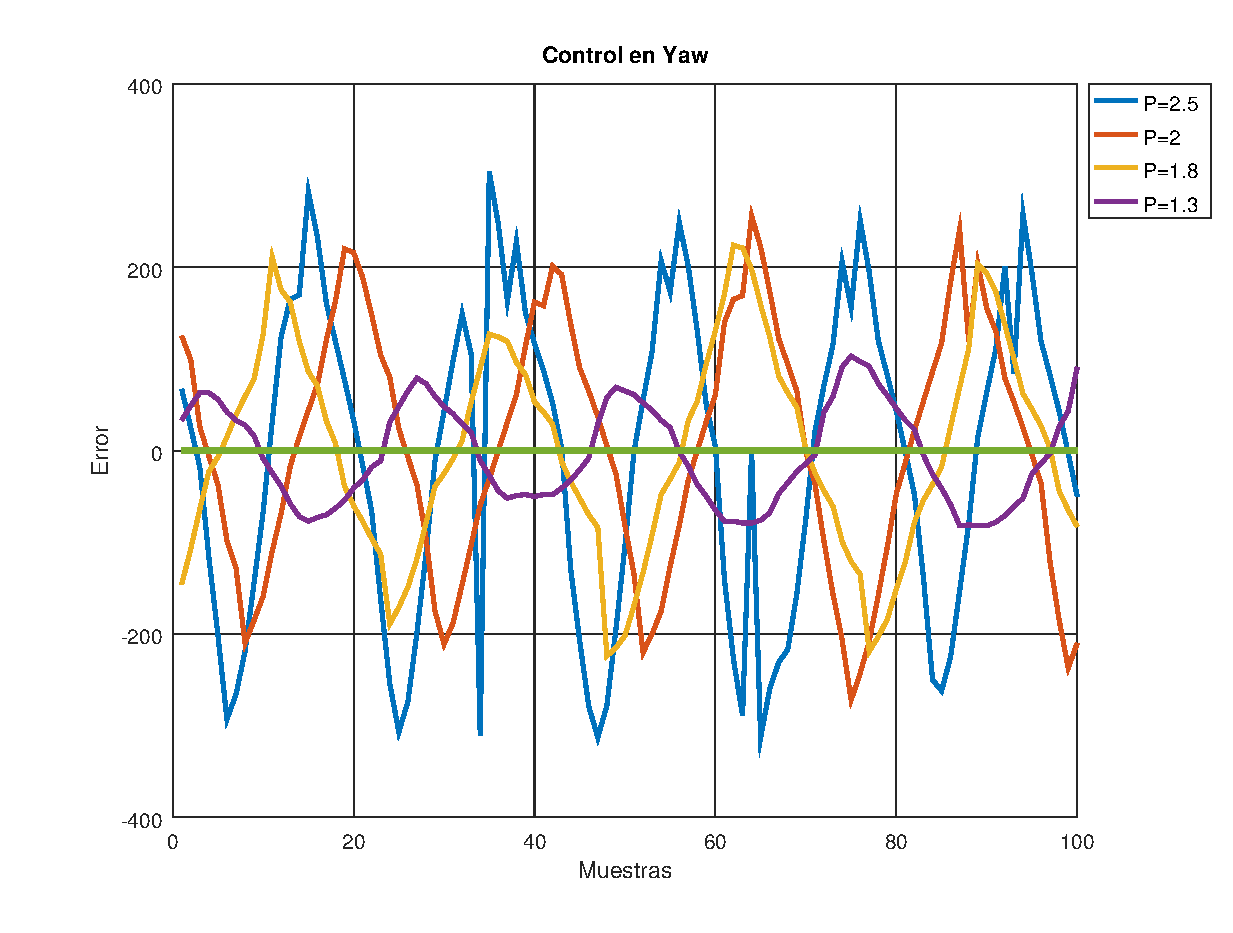
\includegraphics[width=0.75\textwidth]{Contenido/Cuerpo/Capitulo5/Fig8.eps}
	\captionof{figure}{Control proporcional sobre el eje X}\label{Fig4}
\end{center}
El primer control se hizo variando el valor de Kp para poder ver la respuesta de la oscilación del sistema, donde se puede ver claramente que la
frecuencia aumenta conforme la ganancia lo hace, por lo que mete inestabilidad a la lectura.\\
Haciendo el mismo procedimiento en el eje Y variando las ganancias tenemos:
\begin{center}
	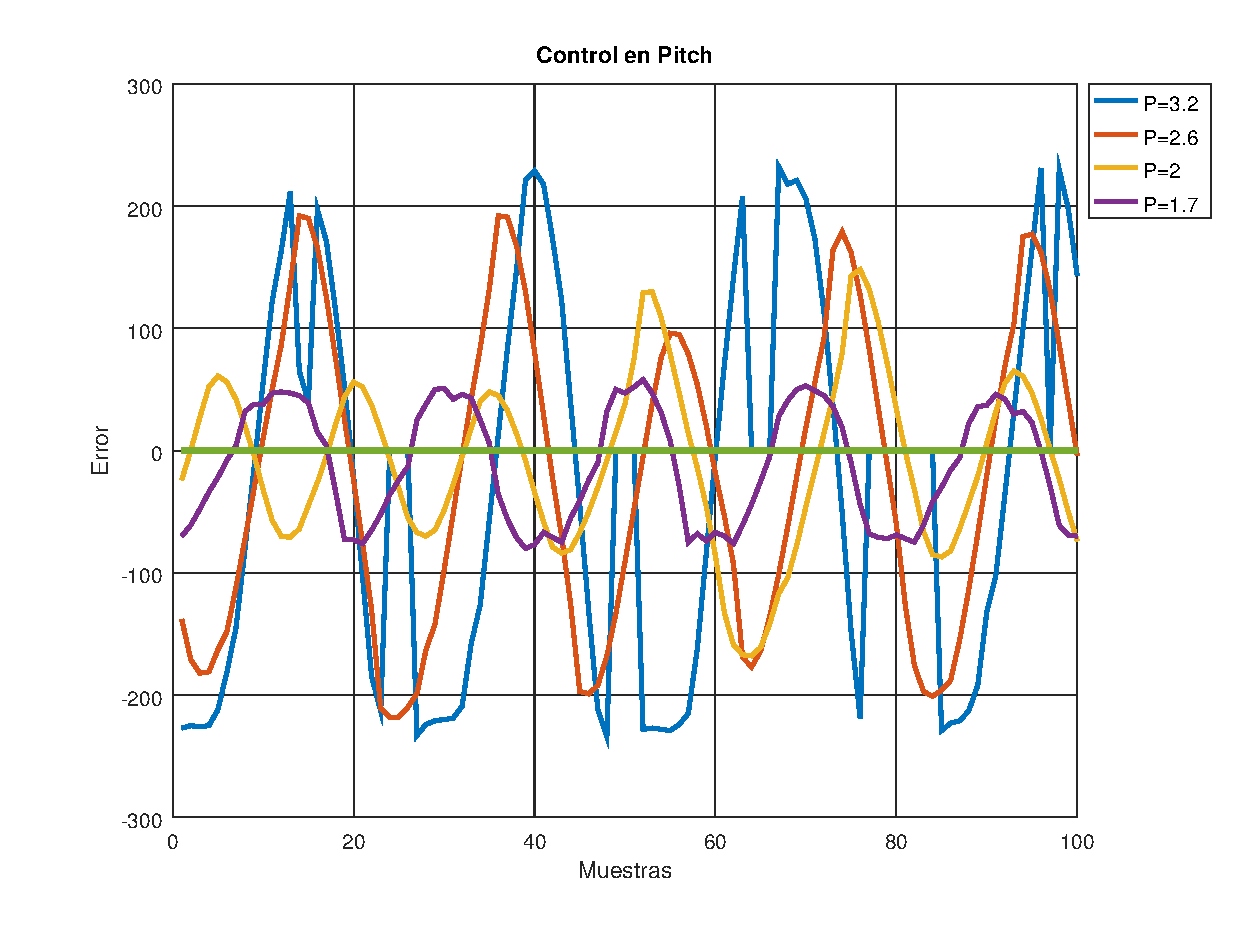
\includegraphics[width=0.75\textwidth]{Contenido/Cuerpo/Capitulo5/Fig9.eps}
	\captionof{figure}{Control proporcional sobre el eje Y}\label{Fig4}
\end{center}
Similar a lo que pasa en X ocurre a Y, donde conforme la oscilación aumenta a un nivel incontrolable.\\
El siguiente paso es reducir las oscilaciones utilizando el control Derivativo, que sirve como amortiguador para tener un mejor control.
Empezando por agregar varios valores de Kd hasta lograr que pueda amortiguar y llegar a un punto donde las oscilaciones sean en estado
estacionario.\\
El metodo de sintonización esta basado en primero hacer oscilar al sistema por medio de la adicion de un control proporcional para despues
amortiguar el sistema agregando un control derivativo, dejando entonces al sistema con pequeñas oscilaciones que pueden ser corregidas con un
control integral. \\
Las siguientes graficas ilustran las variaciones de Kd en el control del Yaw:
\begin{center}
	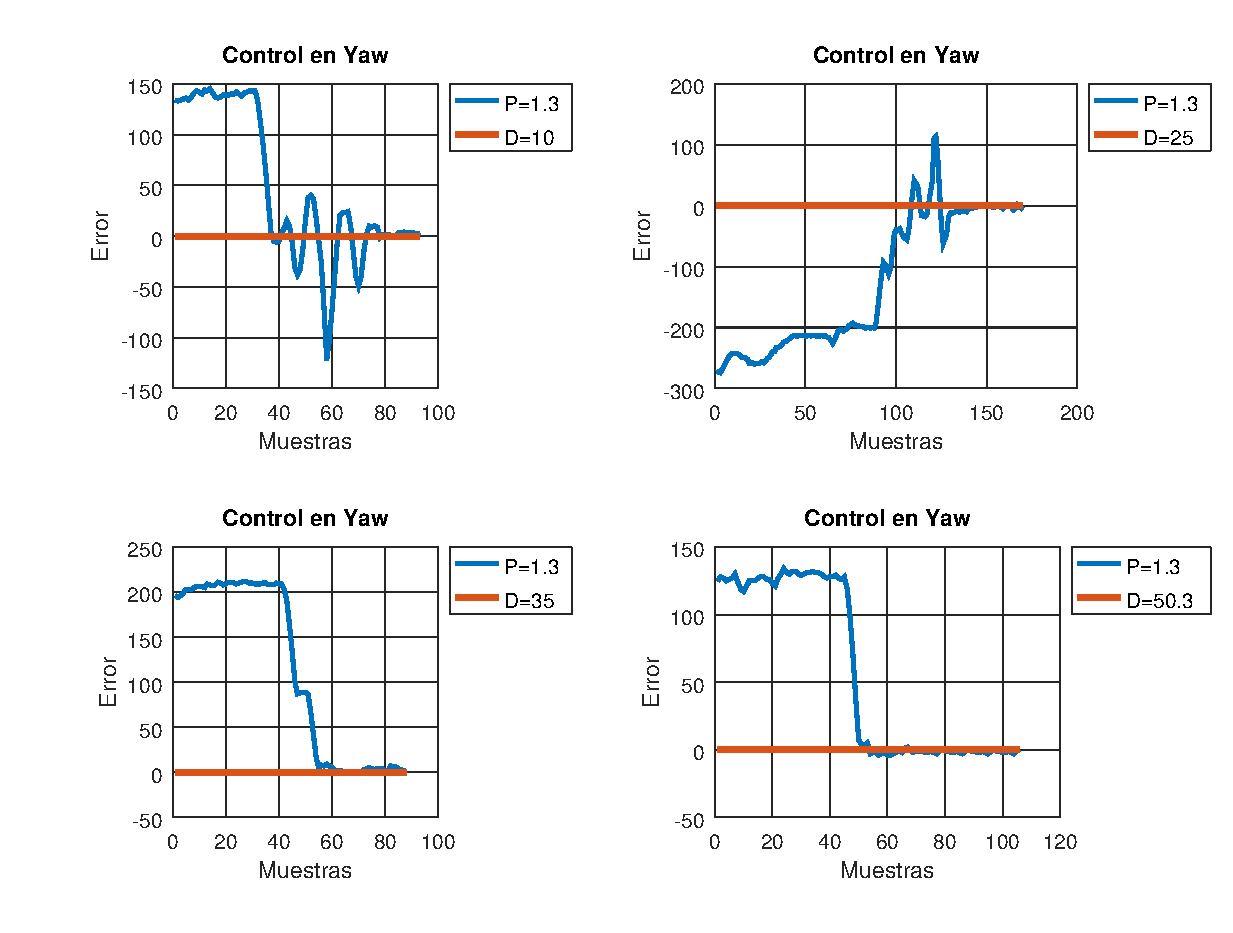
\includegraphics[width=0.9\textwidth]{Contenido/Cuerpo/Capitulo5/Fig10.eps}
	\captionof{figure}{Control proporcional derivativo sobre el eje X}\label{Fig4}
\end{center}
De donde podemos observar como es que la señal es amortiguada a tal nivel que el error se acerca a cero con +-3, que para ser
un error de pixeles se vuelve un control deseado, debido a que la diferencia entre un pixel y otro esta en el orden de los milis.\\
Por su parte tenemos el control en Pitch donde se siguio el mismo procedimiento que en el otro eje descrito.
\begin{center}
	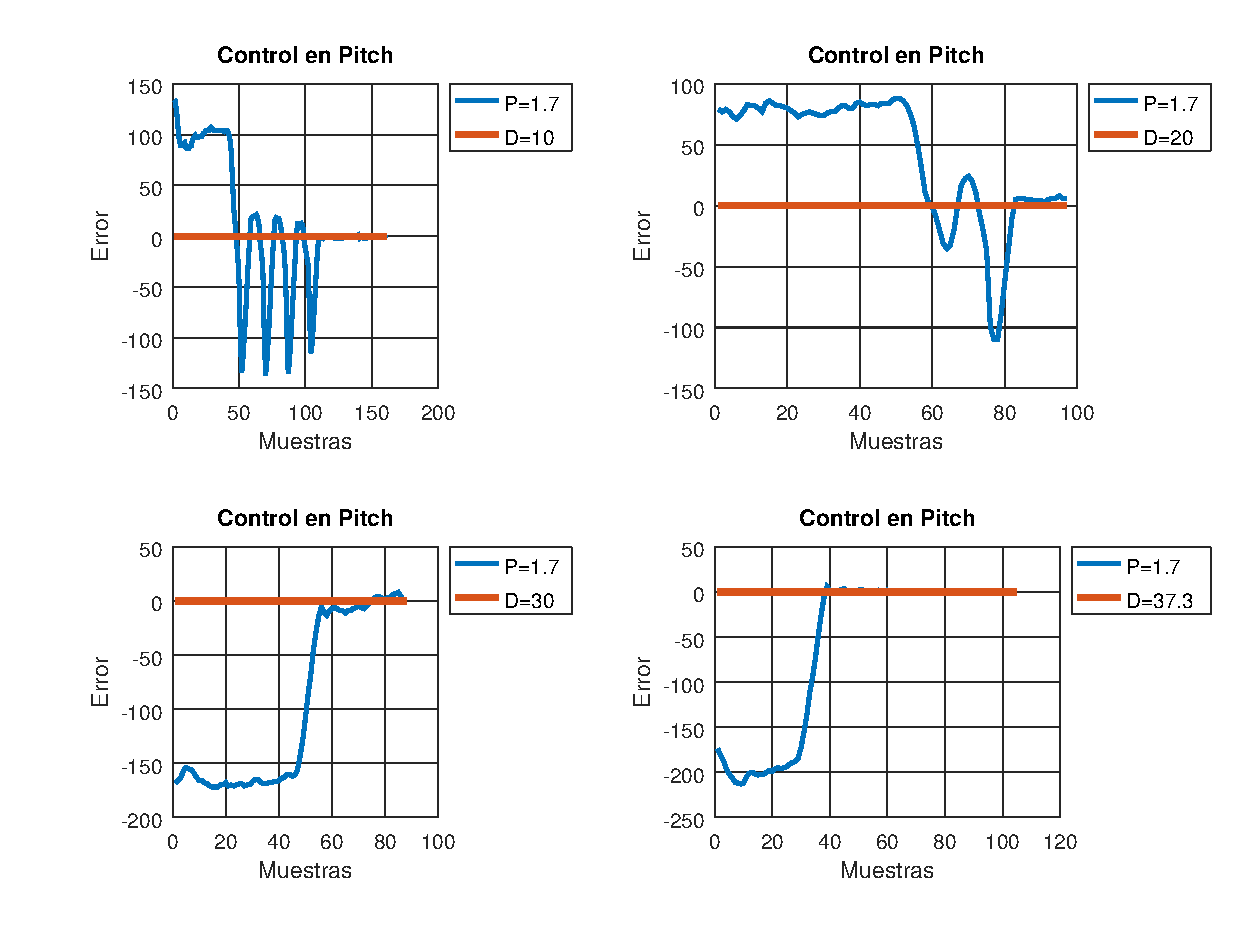
\includegraphics[width=0.8\textwidth]{Contenido/Cuerpo/Capitulo5/Fig11.eps}
	\captionof{figure}{Control proporcional derivativo sobre el eje Y}\label{Fig4}
\end{center}
